\documentclass{scrreprt}

\usepackage{aligned-overset}
\usepackage{amsmath}
\usepackage{amsthm}
\usepackage{amssymb}
\usepackage{bm}
\usepackage[inline, shortlabels]{enumitem}
\usepackage{hyperref}
\usepackage[utf8]{inputenc}
\usepackage{multicol}
\usepackage{mathtools}
\usepackage{pdflscape}
\usepackage{physics}
\usepackage{polynom}
\usepackage{tabularx}
\usepackage[table]{xcolor}
\usepackage{titling}
\usepackage{fancyhdr}
\usepackage{xfrac}
\usepackage{pgfplots}

\pgfplotsset{compat = newest}
\usepgfplotslibrary{fillbetween}
\usetikzlibrary{arrows, arrows.meta}
\usetikzlibrary{calc}
\usetikzlibrary{patterns}

\author{Karsten Lehmann}
\date{WiSe 2024/25}
\title{Übungsblatt 6\\INF-B-110, Diskrete Strukturen}

\setlength{\headheight}{26pt}
\pagestyle{fancy}
\fancyhf{}
\lhead{\thetitle}
\rhead{\theauthor}
\lfoot{\thedate}
\rfoot{Seite \thepage}

\newcommand{\ggT}[0]{\text{ggT}}
\DeclarePairedDelimiter{\floor}{\lfloor}{\rfloor}

\begin{document}

\paragraph{Ü 6.1} Es sei $R$ die Menge aller Symmetrieabbildungen eines
Rechtecks, das kein Quadrat ist.
\begin{enumerate}[(a)]
\item Geben Sie alle diese Symmetrieabbildungen als Permutationen der Eckpunkte
  des Rechtecks an (die Eckpunkte seien gegen den Uhrzeigensinn mit 1, 2, 3, 4
  bezeichnet).

  \subparagraph{Lsg.} Ein nicht-quadratisches Rechteck besitzt die folgenden
  Symmetrieabbildungen:

  \begin{tikzpicture}
    \node[label=above left:1] (1) at (0, 0) {};
    \node[label=below left:2] (2) at (0, -5) {};
    \node[label=below right:3] (3) at (10, -5) {};
    \node[label=above right:4] (4) at (10, 0) {};
    \draw (1.center) -- (2.center) -- (3.center) -- (4.center) -- (1.center);

    \draw[dashed, red!40, line width=0.7mm] (-2, -2.5) -- (12, -2.5);
    \draw[dashed, blue!40, line width=0.7mm] (5, 2) -- (5, -7);

    \draw[->, >=stealth', dashed, green!90!black!40, line width=0.7mm] (4.8, -1.4) arc[radius=1.2, start angle=90, end angle=270];
    \draw[->, >=stealth', dashed, yellow!90!black!80, line width=0.7mm] (5.2, -1.4) arc[radius=1.2, start angle=90, end angle=-90];

    \node[red!60] at (-2, -2) {$\qty\big(1\:2)\qty\big(4\:3)$};
    \node[blue!60] at (4, 2) {$\qty\big(1\:4)\qty\big(2\:3)$};
    \node[green!70!black!90] at (3, -1) {$\qty\big(1\:3)\qty\big(4\:2)$};
    \node[yellow!70!black!90] at (7, -4) {$\qty\big(1\:3)\qty\big(4\:2)$};
  \end{tikzpicture}

  \begin{enumerate}[(1)]
  \item \colorbox{orange!20}{Identitätsabbildung $\text{id}$}
  \item \colorbox{red!20}{Spiegelung an einer horizontalen Achse}
  \item \colorbox{blue!20}{Spiegelung an einer vertikalen Achse}
  \item \colorbox{green!20}{Rotation gegen den Uhrzeigersinn}
  \item \colorbox{yellow!20}{Rotation im Uhrzeigersinn}
  \end{enumerate}
  Wobei die beiden Rotation identisch sind.

\newpage
\item Zeigen Sie, dass $\qty\big(R; \circ)$ mit der Hintereinanderausführung
  $\circ$ von Abbildungen eine Gruppe bildet.
  Stellen Sie dazu die Verknüpfungstafel auf und verwenden Sie diese für Ihre
  Argumentation.

  \subparagraph{Lsg.} Seien
  \colorbox{red!20}{$\qty\big(1\:2) \qty\big(3\:4)$} die horizontale
  Spiegelung, \colorbox{blue!20}{$\qty\big(1\:4)\qty\big(2\:3)$} die
  vertikale Spiegelung, \colorbox{green!20}{$\qty\big(1\:3)\qty\big(4\:2)$}
  die Rotation und \colorbox{orange!20}{$\text{id}$} die Identitätsabbildung.

  \begin{tabular}{|c|cccc|}
    \hline
    $\circ$
    & \colorbox{orange!20}{$\text{id}$}
    & \colorbox{red!20}{$\qty\big(1\:2) \qty\big(3\:4)$}
    & \colorbox{blue!20}{$\qty\big(1\:4)\qty\big(2\:3)$}
    & \colorbox{green!20}{$\qty\big(1\:3)\qty\big(4\:2)$} \\
    \hline
    \colorbox{orange!20}{$\text{id}$}
    & \colorbox{orange!20}{$\text{id}$}
    & \colorbox{red!20}{$\qty\big(1\:2) \qty\big(3\:4)$}
    & \colorbox{blue!20}{$\qty\big(1\:4)\qty\big(2\:3)$}
    & \colorbox{green!20}{$\qty\big(1\:3)\qty\big(4\:2)$} \\
    \colorbox{red!20}{$\qty\big(1\:2) \qty\big(3\:4)$}
    & \colorbox{red!20}{$\qty\big(1\:2) \qty\big(3\:4)$}
    & \colorbox{orange!20}{$\text{id}$}
    & \colorbox{green!20}{$\qty\big(1\:3)\qty\big(4\:2)$}
    & \colorbox{blue!20}{$\qty\big(1\:4)\qty\big(2\:3)$} \\
    \colorbox{blue!20}{$\qty\big(1\:4)\qty\big(2\:3)$}
    & \colorbox{blue!20}{$\qty\big(1\:4)\qty\big(2\:3)$}
    & \colorbox{green!20}{$\qty\big(1\:3)\qty\big(4\:2)$}
    & \colorbox{orange!20}{$\text{id}$}
    & \colorbox{red!20}{$\qty\big(1\:2) \qty\big(3\:4)$} \\
    \colorbox{green!20}{$\qty\big(1\:3)\qty\big(4\:2)$}
    & \colorbox{green!20}{$\qty\big(1\:3)\qty\big(4\:2)$}
    & \colorbox{blue!20}{$\qty\big(1\:4)\qty\big(2\:3)$}
    & \colorbox{red!20}{$\qty\big(1\:2) \qty\big(3\:4)$}
    & \colorbox{orange!20}{$\text{id}$} \\
    \hline
  \end{tabular}
  Für eine Gruppen werden nun benötigt:
  \begin{enumerate}[(1)]
  \item Ein neutrales Element $e$ mit $e \circ r = r = r \circ e$ für alle
    $r \in R$.

    Aus der Verknüpfungstafel kann $\text{id}$ als neutrales Element abgelesen
    werden.

  \item Einem inversen Element $r^{-1} \in R$ für jedes $r \in R$ mit
    $r^{-1} \circ r = r \circ r^{-1} = e$.

    Aus der Verknüpfungstafel kann $r \circ r = \text{id}$ für alle $r \in R$
    abgelesen werden.

  \item Die Assoziativität der Komposition.
    Für $a, b, c \in R$ gilt
    $\qty\big(a \circ b) \circ c = a \circ \qty\big(b \circ c)$.

    Dies kann ebenfalls aus der Verknüpfungstafel abgelesen werden.
  \end{enumerate}

  Somit handelt es sich um eine Gruppe.

\item Ist $\qty\big(R, \circ)$ abelsch?

  \subparagraph{Lsg.} Ein Gruppe heißt abelsch, falls die Verknüpfung
  kommutativ ist, also $a \circ b = b \circ a$ für alle $a, b \in R$.
  Und auch dies kann der Verknüpfungstafel entnommen werden.
  Somit ist die Gruppe tatsächlich abelsch.
\end{enumerate}

\paragraph{Ü 6.2}
\begin{enumerate}[(a)]
\item Es sei $\qty\big(G; \circ)$ eine Gruppe mit neutralem Element $e$.
  Beweisen Sie die Kürzungsregeln:
  \[
    \forall a, b, c \in G \colon
    a \circ b = a \circ c \Rightarrow b = c
    \text{ und }
    b \circ a = c \circ a \Rightarrow b = c
  \]

  \subparagraph{Lsg.} Sei $a \circ b = a \circ c$.
  Dann ist
  \begin{flalign*}
    a^{-1} \circ \qty\big(a \circ b) &= a^{-1} \circ \qty\big(a \circ c) & \overset{\text{Assoziativität}}&\iff \\
    \qty\big(a^{-1} \circ a) \circ b &= \qty\big(a^{-1} \circ a) \circ c & \overset{\text{Inverses}}&\iff \\
    e \circ b &= e \circ c & \overset{\text{Neutrales Element}}&\iff \\
    b &= c
  \end{flalign*}

  Sei $b \circ a = c \circ a$.
  Dann ist
  \begin{flalign*}
    \qty\big(b \circ a) \circ a^{-1} &= \qty\big(c \circ a) \circ a^{-1} & \overset{\text{Assoziativität}}&\iff \\
    b \circ \qty\big(a \circ a^{-1}) &= c \circ \qty\big(a \circ a^{-1}) & \overset{\text{Inverses}}&\iff \\
    b \circ e &= c \circ e & \overset{\text{Neutrales Element}}&\iff \\
    b &= c
  \end{flalign*}

\item Zeigen Sie, dass für jede endliche Gruppe $\qty\big(G; \circ)$ gilt:
  In der Verknüpfungstafel tritt in jeder Zeile und in jeder Spalte jedes
  Element der Gruppe genau einmal auf.

  \subparagraph{Lsg.} Angenommen ein Element $x \in G$ würde in einer Zeile
  und/oder Spalte der Verknüpfungstafel zweimal vorkommen.
  Dann existieren paarweise verschiedene Elemente $a, b, c \in G$ mit
  $a \circ b = x = a \circ c$ und/oder $b \circ a = x = c \circ a$.
  Ein Widerspruch zur Teilaufgabe (a).

  \textbf{Alternativ nach der Übung:} Sei $g \in G$.
  In der zu $g$ zugehörigen Spalte stehen genau die Elemente $\qty\big{h \circ g \:\big|\: h \in G}$.

  Die Abbildung $G \to G, h \mapsto h_g$ ist injektiv $\Rightarrow$ jedes Element höchstens einmal

  Da $G$ endlich, ist die Abbildung bijektiv $\Rightarrow$ jedes Element genau einmal.

  \underline{Bemerkung:} $G \to G, h \mapsto h_g$ ist immer bijektiv.
  Denn sei $a \in G$.
  Dann ist $h \circ \qty\big(h^{-1} \circ a) = \qty\big(h \circ h^{-1}) \circ a = a$.
  Also gibt es $g \in G$ mit $h_g = a$, nämlich $g = h^{-1} \circ a$.
\end{enumerate}

\paragraph{Ü 6.3} Stellen Sie für folgende Gruppen die Verknüpfungstafeln auf:
\begin{enumerate}[(i)]
\item $\qty\big(\mathbb{Z}_4; +)$
\item $\qty\big(\mathbb{Z}_2 \times \mathbb{Z}_2; +)$
  (mit komponentenweiser Addition mod 2)
\item $\qty\big(\mathbb{Z}_7 \setminus \qty\big{0}; \cdot)$
\end{enumerate}
Geben Sie jeweils das neutrale Element und zu jedem Element sein Inverses an.

\subparagraph{Lsg.}
\begin{enumerate}[(i)]
\item Es ist

  \begin{tabular}{|c|cccc|}
    \hline
    + & 0 & 1 & 2 & 3 \\
    \hline
    0 & 0 & 1 & 2 & 3 \\
    1 & 1 & 2 & 3 & 0 \\
    2 & 2 & 3 & 0 & 1 \\
    3 & 3 & 0 & 1 & 2 \\
    \hline
  \end{tabular}

  mit $0$ als neutralem Element und den inversen Elementen

  \begin{enumerate*}[\null]
  \item $0$ für $0$,
  \item $3$ für $1$,
  \item $2$ für $2$,
  \item $1$ für $3$
  \end{enumerate*}

\item Es ist

  \begin{tabular}{|c|cccc|}
    \hline
    +
    & $\begin{pmatrix} 0 \\ 0 \end{pmatrix}$
    & $\begin{pmatrix} 0 \\ 1 \end{pmatrix}$
    & $\begin{pmatrix} 1 \\ 0 \end{pmatrix}$
    & $\begin{pmatrix} 1 \\ 1 \end{pmatrix}$ \\
    \hline
    $\begin{pmatrix} 0 \\ 0 \end{pmatrix}$
    & $\begin{pmatrix} 0 \\ 0 \end{pmatrix}$
    & $\begin{pmatrix} 0 \\ 1 \end{pmatrix}$
    & $\begin{pmatrix} 1 \\ 0 \end{pmatrix}$
    & $\begin{pmatrix} 1 \\ 1 \end{pmatrix}$ \\
    $\begin{pmatrix} 0 \\ 1 \end{pmatrix}$
    & $\begin{pmatrix} 0 \\ 1 \end{pmatrix}$
    & $\begin{pmatrix} 0 \\ 0 \end{pmatrix}$
    & $\begin{pmatrix} 1 \\ 1 \end{pmatrix}$
    & $\begin{pmatrix} 1 \\ 0 \end{pmatrix}$ \\
    $\begin{pmatrix} 1 \\ 0 \end{pmatrix}$
    & $\begin{pmatrix} 1 \\ 0 \end{pmatrix}$
    & $\begin{pmatrix} 1 \\ 1 \end{pmatrix}$
    & $\begin{pmatrix} 0 \\ 0 \end{pmatrix}$
    & $\begin{pmatrix} 0 \\ 1 \end{pmatrix}$ \\
    $\begin{pmatrix} 1 \\ 1 \end{pmatrix}$
    & $\begin{pmatrix} 1 \\ 1 \end{pmatrix}$
    & $\begin{pmatrix} 1 \\ 0 \end{pmatrix}$
    & $\begin{pmatrix} 0 \\ 1 \end{pmatrix}$
    & $\begin{pmatrix} 0 \\ 0 \end{pmatrix}$ \\
    \hline
  \end{tabular}

  mit $\begin{pmatrix} 0 \\ 0 \end{pmatrix}$ als neutralem Element und den
  inversen Elementen

  \begin{enumerate*}[\null]
  \item $\begin{pmatrix} 0 \\ 0 \end{pmatrix}$
    für $\begin{pmatrix} 0 \\ 0 \end{pmatrix}$,
  \item $\begin{pmatrix} 0 \\ 1 \end{pmatrix}$
    für $\begin{pmatrix} 0 \\ 1 \end{pmatrix}$,
  \item $\begin{pmatrix} 1 \\ 0 \end{pmatrix}$
    für $\begin{pmatrix} 1 \\ 0 \end{pmatrix}$,
  \item $\begin{pmatrix} 1 \\ 1 \end{pmatrix}$
    für $\begin{pmatrix} 1 \\ 1 \end{pmatrix}$
  \end{enumerate*}

\item Es ist

  \begin{tabular}{|c|cccccc|}
    \hline
    $\cdot$ & 1 & 2 & 3 & 4 & 5 & 6 \\
    \hline
    1 & 1 & 2 & 3 & 4 & 5 & 6 \\
    2 & 2 & 4 & 6 & 1 & 3 & 5 \\
    3 & 3 & 6 & 2 & 5 & 1 & 4 \\
    4 & 4 & 1 & 5 & 2 & 6 & 3 \\
    5 & 5 & 3 & 1 & 6 & 4 & 2 \\
    6 & 6 & 5 & 4 & 3 & 2 & 1 \\
    \hline
  \end{tabular}

  mit $1$ als neutralem Element und den inversen Elementen
  \begin{itemize}
  \item $1$ für $1$
  \item $4$ für $2$
  \item $5$ für $3$
  \item $2$ für $4$
  \item $3$ für $5$
  \item $6$ für $6$
  \end{itemize}
\end{enumerate}

\newpage
\paragraph{Ü 6.4} Welche der Elemente $z_1 = 7$, $z_2 = 8$, $z_3 = 13$ und
$z_4 = 15$ aus $\mathbb{Z}_{24}$ sind Nullteiler, welche sind Einheiten?
Bestimmen Sie für diese Elemente - wenn möglich - das multiplikative Inverse in
$\mathbb{Z}_{24}$.
Verwenden Sie dazu den erweiterten euklidischen Algorithmus.

\subparagraph{Lsg.} Ein Element $a \in \mathbb{Z}_{24}$ heißt Nullteiler, falls
$b \in \mathbb{Z}_{24}$ mit $a \cdot b = 0$ existiert.

Das ist genau dann der Fall, wenn ein Primfaktor von $a$ ein Teiler von 24
ist, da dann $a = p \cdot y$ und $24 = p \cdot z$ mit $y$ und $z$ als
Produkt der restlichen Primfaktoren von $a$ und 24, sowie
$a \cdot z = p \cdot y \cdot z = p \cdot z \cdot y = 24 \cdot y \equiv 0 (\mod 24)$

Somit sind $z_2 = 8$ und $z_4 = 15$ Nullteiler mit $3 \cdot 8 = 0$ und
$8 \cdot 15 = 0$.

In der Vorlesung wurde bereits bewiesen, dass ein Nullteiler keine Einheit sein
kann.
Somit müssen lediglich 7 und 13 betrachtet werden.
Nun sind $7 \cdot 7 = 1$ und $13 \cdot 13 = 1$.

Bestimme $\ggT\qty\big(7, 24)$ mit dem erweiterten Euklidischen Algorithmus

\begin{tikzpicture}
  \node[anchor=west] at (0,0) {Es ist nicht $7|24$, also berechne E-EUKLID$\qty\big(24 \mod 7, 7)$};
  \node[anchor=west] at (1.5,-.7) {Es ist nicht $3|7$, also berechne E-EUKLID$\qty\big(7 \mod 3, 3)$};
  \node[anchor=west] at (3,-1.4) {Es ist $1|3$, also gib \hspace{.9cm} zurück};
  \node[anchor=center] (ab2) at (6.8, -1.4) {$\qty\big(1, 0)$};

  \node[anchor=west] at (1.5, -2.6) {Setze \hspace{2.4cm} und gib \hspace{2.5cm} zurück};
  \node[anchor=west] (res1) at (2.5, -2.6) {$a' = 1, b' = 0$};
  \node[anchor=center] (ab1) at (7.8, -2.6) {$\qty(0 - 1 \floor{\frac{7}{3}}, 1)$};

  \node[anchor=west] at (0, -3.8) {Setze \hspace{2.4cm} und gib \hspace{2.6cm} zurück};
  \node[anchor=west] (res0) at (1, -3.8) {$a' = -2, b' = 1$};
  \node[anchor=center] (ab0) at (6.4, -3.8) {$\qty(1 + 2 \floor{\frac{24}{7}}, -2)$};

  \node[anchor=west] at (0, -5) {Somit ist \hspace{2.6cm} und $\ggT\qty\big(7, 24) = 7 \cdot 7 + 24 \cdot (-2) = 1$};
  \node[anchor=west] (res) at (1.8, -5) {$a = 7, b = -2$};

  \draw[->] (ab2) |- ($(res1)!0.5!(ab2)$) -| (res1);
  \draw[->] (ab1) |- ($(res0)!0.5!(ab1)$) -| (res0);
  \draw[->] (ab0) |- ($(res)!0.5!(ab0)$) -| (res);
\end{tikzpicture}

\textbf{Alternativ nach der Übung:} Es ist
\begin{flalign*}
  24 &= 3 \cdot \underline{7} + 3 \\
  7 &= 2 \cdot \underline{3} + 1 \\
  3 &= 1 \cdot 3 + 0
\end{flalign*}
Weiter ist
\begin{flalign*}
  1 &= 1 \cdot 7 - 2 \cdot 3 \\
    &= 1 \cdot 7 - 2 \cdot \qty\big(24 - 3 \cdot 7) \\
    &= 7 \cdot 7 - 2 \cdot 24
\end{flalign*}

Oder

\begin{tabular}{c|cc}
     & 24 & 7 \\
  \hline
  24 & 1 & 0 \\
  7  & 0 & 1 \\
  \hline
  $24 \mod 7 = 3$ & 1 & -3 \\
  $7 \mod 3 = 1$ & -2 & 7
\end{tabular}

\newpage
Bestimme $\ggT\qty\big(13, 24)$ mit dem erweiterten Euklidischen Algorithmus

\begin{tikzpicture}
  \node[anchor=west] at (0,0) {Es ist nicht $13|24$, also berechne E-EUKLID$\qty\big(24 \mod 13, 13)$};
  \node[anchor=west] at (1.5,-.7) {Es ist nicht $11|13$, also berechne E-EUKLID$\qty\big(13 \mod 11, 11)$};
  \node[anchor=west] at (3,-1.4) {Es ist nicht $2|11$, also berechne E-EUKLID$\qty\big(11 \mod 2, 2)$};
  \node[anchor=west] at (4.5,-2.1) {Es ist $1|2$, also gib \hspace{.9cm} zurück};
  \node[anchor=center] (ab3) at (8.3, -2.1) {$\qty\big(1, 0)$};

  \node[anchor=west] at (3, -3.2) {Setze \hspace{2.1cm} und gib \hspace{2.2cm} zurück};
  \node[anchor=west] (res2) at (4, -3.2) {$a' = 1, b' = 0$};
  \node[anchor=center] (ab2) at (9, -3.2) {$\qty(0 - 1 \floor{\frac{11}{2}}, 1)$};

  \node[anchor=west] at (1.5, -4.4) {Setze \hspace{2.4cm} und gib \hspace{2.5cm} zurück};
  \node[anchor=west] (res1) at (2.5, -4.4) {$a' = -5, b' = 1$};
  \node[anchor=center] (ab1) at (7.8, -4.4) {$\qty(1 + 5 \floor{\frac{13}{11}}, -5)$};

  \node[anchor=west] at (0, -5.6) {Setze \hspace{2.4cm} und gib \hspace{2.6cm} zurück};
  \node[anchor=west] (res0) at (1, -5.6) {$a' = 6, b' = -5$};
  \node[anchor=center] (ab0) at (6.4, -5.6) {$\qty(-5 - 6 \floor{\frac{24}{13}}, 6)$};

  \node[anchor=west] at (0, -6.8) {Somit ist \hspace{2.6cm} und $\ggT\qty\big(13, 24) = 13 \cdot (-11) + 6 \cdot 24 = 1$};
  \node[anchor=west] (res) at (1.8, -6.8) {$a = -11, b = 6$};

  \draw[->] (ab3) |- ($(res2)!0.5!(ab3)$) -| (res2);
  \draw[->] (ab2) |- ($(res1)!0.5!(ab2)$) -| (res1);
  \draw[->] (ab1) |- ($(res0)!0.5!(ab1)$) -| (res0);
  \draw[->] (ab0) |- ($(res)!0.5!(ab0)$) -| (res);
\end{tikzpicture}

(Und $-11 \equiv 13 \qty\big(\mod 24)$)

\textbf{Alternativ nach der Übung:} Es ist
\begin{flalign*}
  24 &= 1 \cdot \underline{13} + 11 \\
  13 &= 1 \cdot \underline{11} + 2 \\
  11 &= 5 \cdot \underline{2} + 1 \\
  2 &= 2 \cdot 1 + 0
\end{flalign*}
Weiter ist
\begin{flalign*}
  1 &= 1 \cdot 11 - 5 \cdot 2 \\
    &= 1 \cdot 11 - 5 \cdot \qty\big(13 - 1 \cdot 11) \\
    &= 6 \cdot 11 - 5 \cdot 13 \\
    &= 6 \cdot \qty\big(24 - 1 \cdot 13) - 5 \cdot 13 \\
    &= 6 \cdot 24 - 11 \cdot 13 \\
\end{flalign*}
\end{document}
